%% The following is a directive for TeXShop to indicate the main file
%%!TEX root =../diss.tex

\chapter{Future Work}
\label{ch:futurework}

The work presented in this chapter are a collection of preliminary results, alternative analysis methods, and proposed future work. 
\SARi{you couldn't make it less appealing. This sounds like and odds-and-sods sort of chapter. please market more convincingly. don't use the word collection}

\section{Group-ICA}

One of the principal limitations of \acs{ICA} is that it ``does not naturally generalize to a method suitable for drawing inferences about groups of subjects~\cite{Calhoun:2009jr}.
In this thesis, we developed a quantification method to mitigate this issue by comparing component weighting factor strength after normalization (Section~\ref{sec:correctionfactor}).
Calhoun et al., has reviewed several methods for analyzing multiple subjects within a cohort using \acs{ICA} have been proposed~\cite{Calhoun:2009jr}.
The approach that is most relevant for the data collected for the experiments presented in this thesis (section~\ref{sec:B20_expt1}) is spatial concatenation~\cite{Calhoun:2001jx}.
Briefly, cohort data for groupICA was constructed by concatenating all 16 slices from the 17 subjects together in the z-dimension.
Figure~\ref{groupICAschematic} compares group ICA to the standard ICA technique described in Chapter~\ref{ch:oemri1}.
The same deflation-based \acs{FastICA} (python package \texttt{scikit.sklearn}~v0.17.1) was used to analyze the data.
To ensure the cyclic behaviour of the T$_1$ weighted signal intensity corresponding to the gas challenge appeared in only one component, the number of independent components was set to 9.
Application of \acs{ICA} to the spatially concatenated data produced a single oxygen-enhancing component that matched the temporal pattern of the gas cycling paradigm in all 17 animals (Figure~\ref{groupICA1}). 
This component appears to be smoother than typical extracted oxygen enhancing components because it represents the group response rather than the individual features that exist in each mouse that responds somewhat differently.

\begin{figure}[htbp]
   \centering
   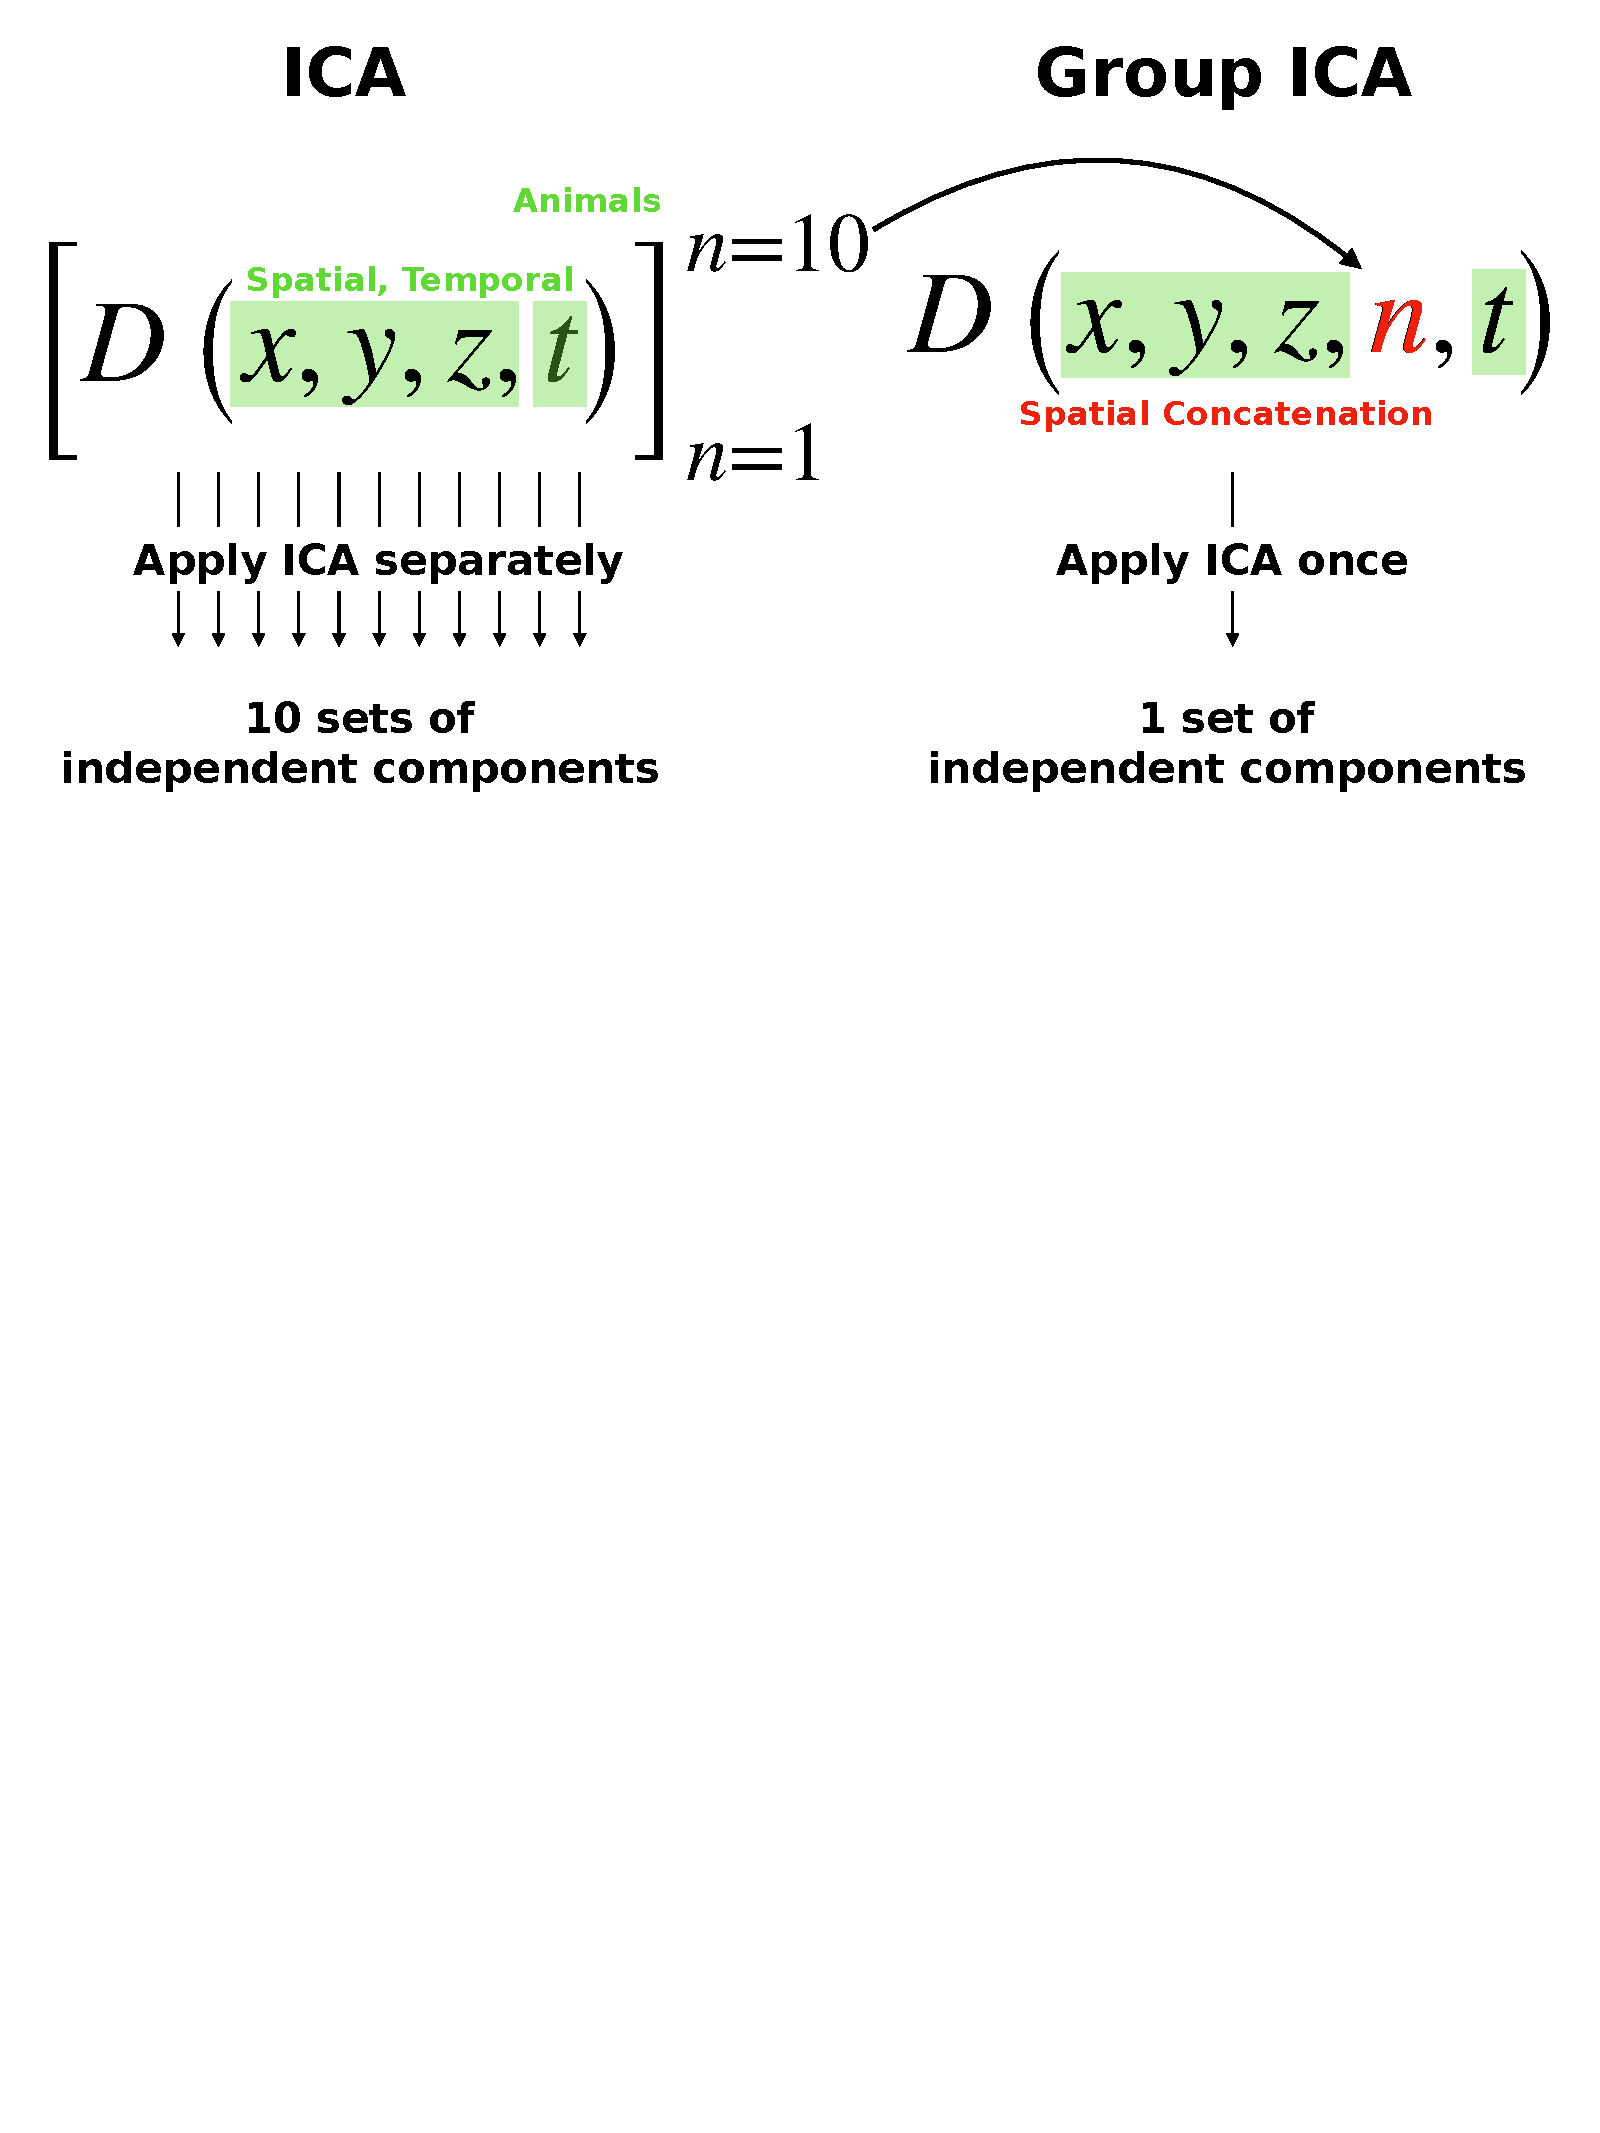
\includegraphics[width=\textwidth]{futurework/futurework-images/groupICA_schematic.pdf} % requires the graphicx package
   \caption{Comparison of the standard ICA technique and groupICA. The main difference is in the pre-processing of the MRI data comprising spatial coordinates ($x,y,z$) and temporal information ($t$). GroupICA datasets are prepared by spatially concatenating all animals together ($n$). The output of the ICA techniques also differs: in standard ICA each application produces a set of independent components whereas in groupICA only a single set of independent components is produced.
   \label{groupICAschematic}}
\end{figure}

Upon selection of the single oxygen enhancing component, reshaping the resultant weighting-factor maps to the original matrix size provided inter-subject comparable data.
Final normalized \acs{dOE-MRI} maps were obtained by dividing each pixel of the component map for each animal with the mean signal-intensity over time of the corresponding pixel in the dOE-MRI scan.
Corresponding \acs{dOE-MRI} are comparable to the methods presented in Chapter~\ref{ch:oemri3} and conclusions of the B20 effect still hold with this analysis method.

\begin{figure}[htbp]
   \centering
   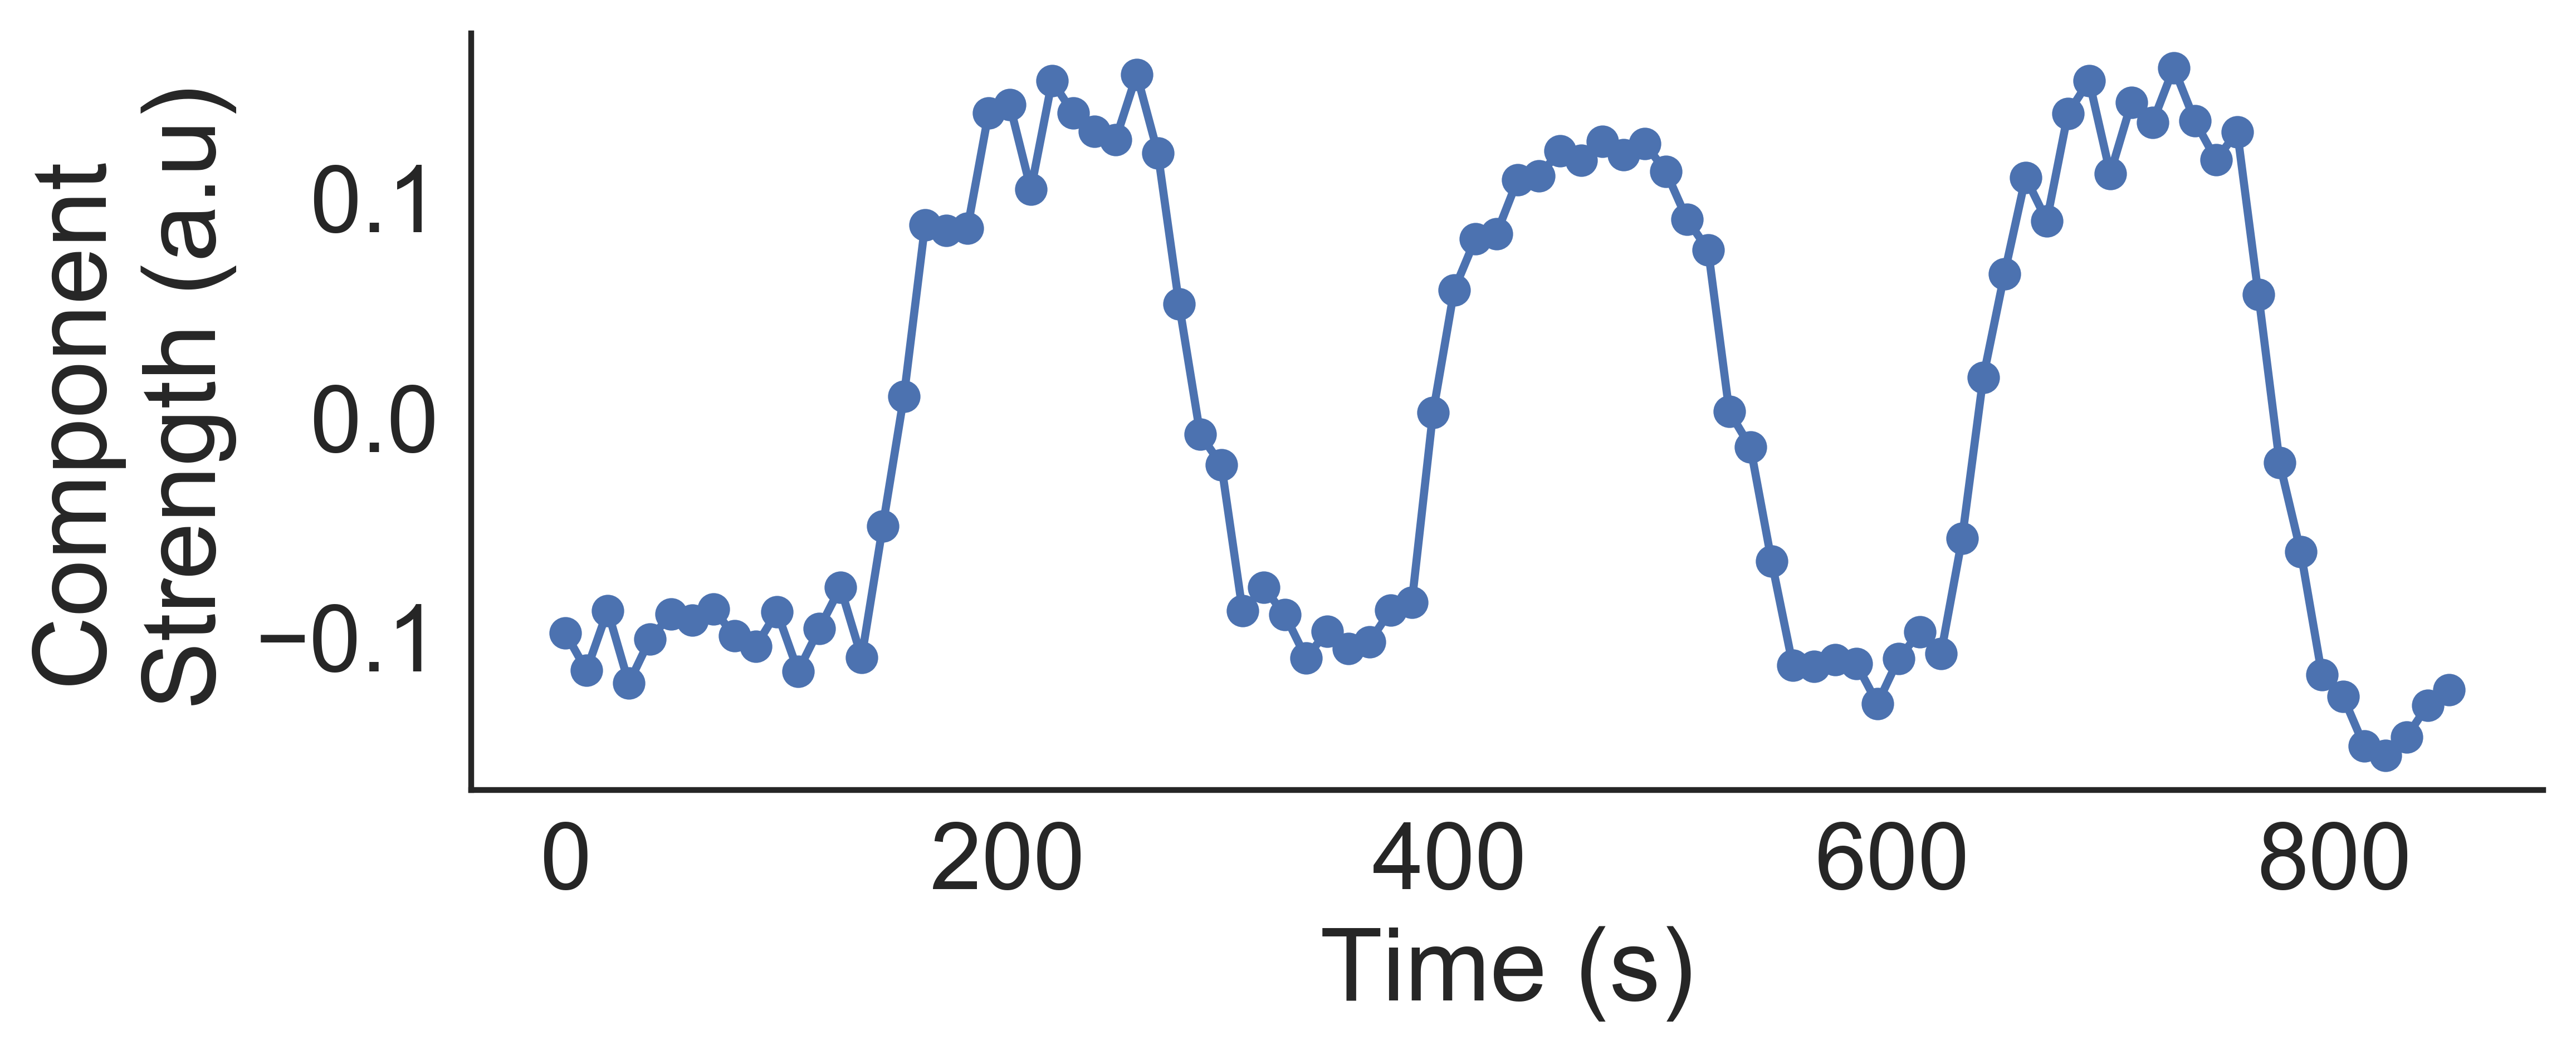
\includegraphics[width=\textwidth]{futurework/futurework-images/ISMRM2019_AARTS3_groupICA_OEcomponent.png} % requires the graphicx package
   \caption{Extracted oxygen enhancing component from \acs{ICA} applied to the spatially concatenated cohort data. One major disadvantage of applying \acs{ICA} only once to multiple animals is that the extracted component averages out any individual features.
   \label{groupICA1}}
\end{figure}

\subsection{Further investigation of the characteristic oxygen response curve}

In this thesis a limited number of tumours models were studied (SCCVII, BT-474, and HCT-116) so it was difficult to generalize whether modeling of the oxygen response curve is characteristic of the tumour environment or model. 
In section~\ref{sec:lognormalfitting_results} we observed that $\sigma_f$ in the SCCVII tumours discriminated between the rapidly growing SCCVII tumours and the other two models.
Further work should include characterizing additional tumour models with varying tumour microenvironments, and also comparison of the oxygen signal decay curves (i.e. when the gas is switched back to room air) as well as the enhancement curves.

\section{dOE-MRI maps of 10 consecutive air/\texorpdfstring{O$_2$}{O2} switches are stable}

The presence of hypoxia in tumours is known to exhibit microregional and temporal heterogeneity.
The process of cells going through periods of oxygen-starvation and then subsequently being re-oxygenated has been termed cyclic hypoxia~\cite{Dewhirst:2009de,Bayer:2011js, Bayer:2012kb}.
A leading cause of cycling hypoxia is the variable flux of red blood cells through the abnormal tumour vasculature on time scales of minutes to hours.
There is some evidence of as there are clear mismatches between pimonidazole staining and perfusion markers (Figure~\ref{fig_perfusion}).
The SCCVII tumour model has specifically been shown to be afflicted by cycling hypoxia as early as  1986~\cite{Chaplin:1986iz}.
It is therefore not surprising that \acs{dOE-MRI} is sensitive to these changes in this tumour model, and provides the first non-invasive data suggesting cycling hypoxia on the relatively short timeline of less than 15 minutes.
The clinical importance of intermittent hypoxia is unclear largely due to poor availability of techniques to measure it in humans~\cite{Michiels:2016hv}. 
Recent work on measuring cycling hypoxia in patients using R$_2^*$~\cite{Panek:2017ge} shows that interest in this phenomenon continues.

Despite the presence of cycling hypoxia in many regions of the SCCVII tumours, O$_2$-enhancing regions in \acs{dOE-MRI} maps are generally in agreement with well perfused areas of histology images.
In particular, concentrated oxygen-responsive regions within a \acs{dOE-MRI} map correspond to highly vascular, perfused regions in matching histology images.
Voxels anti-correlated with the O$_2$ stimulus (O$_2$ refractory, green) typically correspond with pimonidazole staining but there are instances of mismatch (Figures~\ref{fig_sccvii}, ~\ref{fig_hct116}, and ~\ref{fig_perfusion}).
In addition to cycling hypoxia, there may be possible mismatch between the sensitivities of pimonidazole and dOE-MRI and other oxygen sensing modalities (described in \highlight[comment={no ref?}]{Horsman et al.\ NRC 2012)}.
Success of dOE-MRI will ultimately depend on its validation as a clinically useful measure of tumour hypoxia.

To assess this phenomenon, a pilot study was carried out to determine whether this cycling hypoxia can be measured with \acs{dOE-MRI}.
In a small pilot cohort of SCCVII xenografts mice ($n=2$), rather than the standard protocol of three cycles of air-oxygen switches, ten consecutive air-oxygen switches were used.
\acs{ICA} was applied to each cycle of the sequences separately (as described in section~\ref{fig_repeatability}).
Figure~\ref{longcycles} shows the results from a tumour including a \acs{dOE-MRI} map (\ref{longcycles}A), a standard deviation map (\ref{longcycles}B), and a coefficient of variation map (\ref{longcycles}C).
The standard deviation and coefficient of variation maps are surrogate measures of cycling hypoxia as they highlight regions of the tumour that show the highest degree of deviation or variation over the ten cycles.
It is expected that if cycling hypoxia exists, these measures would show regions where it is apparent. 
If cycling hypoxia is not present, then the two parameter maps would be largely feature-less.
In this case, there appears to be little evidence for cycling hypoxia as the \acs{dOE-MRI} maps are fairly consistent from cycle to cycle.
Unfortunately, these results remain un-validated because we were not able to assess cycling hypoxia using histology.
One way to assess cycling hypoxia using histology is to use two separate hypoxia stains (such as EF5 and pimonidazole) and inject them intravenously 30-60 minutes apart.
Imaging the two stains and mapping the differences could confirm the presence or absence of cycling hypoxia. 
A subsequent experiment where the \acs{dOE-MRI} analysis is repeated in more animals alongside the dual hypoxia histological markers would help confirm this finding.
\SARi{Not sure whey B and C show different results. Shouldn't they be very comparable? There is the diagonal ridge in C that's missing on B.}

\begin{figure}[htbp]  
   \centering
   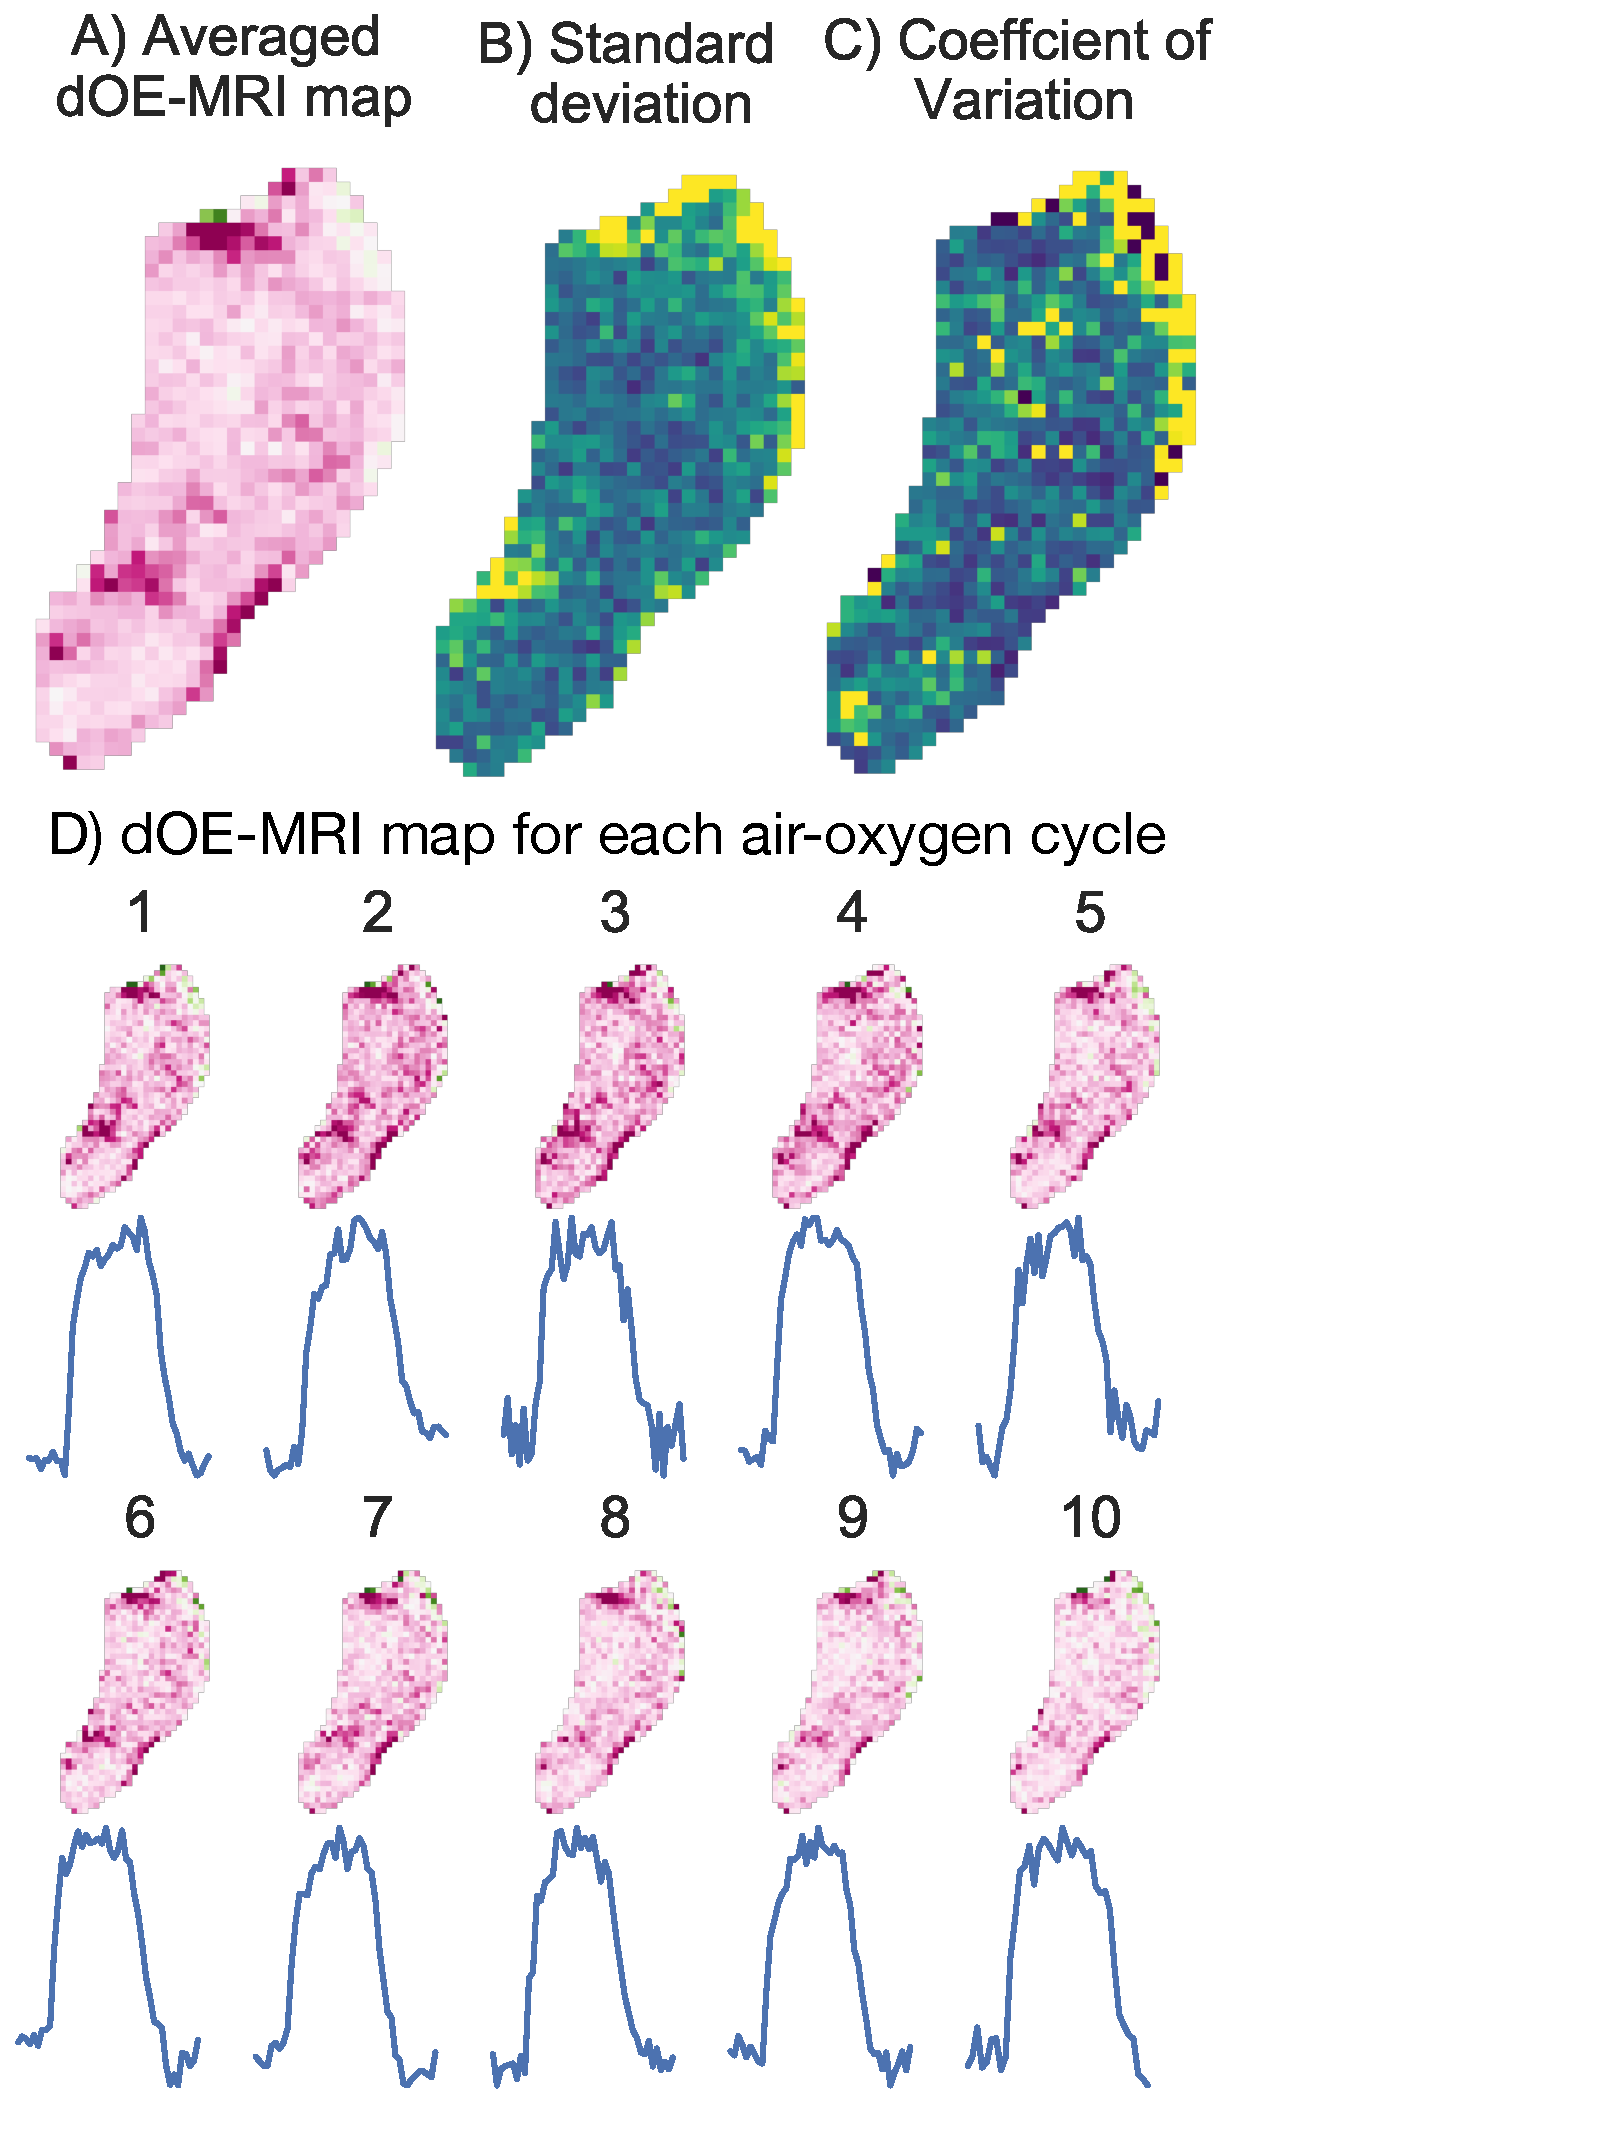
\includegraphics[width=\textwidth]{futurework/futurework-images/cyclingHypoxia.pdf} % requires the graphicx package
   \caption{Results of a \acs{dOE-MRI}-based analysis to sequentially analyze ten consecutive air-oxygen switches (D). The averaged \acs{dOE-MRI} map (A) across all 10 cycles reveals some hyperintense regions corresponding to oxygen-responsive areas. The voxel-wise standard deviation (B) and coefficient of variation (C) of the ten \acs{dOE-MRI} maps shows some variability at the top of the tumour as well as on the mid-right of the tumour.}
   \label{longcycles}
\end{figure}

\section{Exploring the link between perfusion and oxygenation}

One SCCVII and one HCT-116 tumour-bearing mouse were catheterized and injected with 30-mM solution of Gd-DTPA for \acs{DCE-MRI} at a rate of 1~mL/min using a power injector at a dose of 5~$\mu$L/g.

\noindent\textbf{Perfusion maps:} Signal intensity timecourse from the DCE-MRI map was first normalized to the mean signal intensity pre-injection.
Area under the first 60 seconds of the normalized signal intensity enhancement curve after the injection was calculated (\acs{AUC}$_{60}$) using the composite Simpson's Rule (\texttt{scipy.integrate.simps}).
A binary ground-truth perfusion map was constructed by classifying all voxels with AUC$_{60} > 0$ as perfused and everything else as unperfused.

Where \ac{dOE-MRI} and DCE-MRI scans were acquired in the same SCCVII and HCT-116 tumour-bearing mice,  maps of oxygenation status were compared to \acs{AUC}$_{60}$ perfusion maps, as shown in Figure~\ref{fig_perfusion}.
Mean \acs{AUC}$_{60}$ for the well-perfused SCCVII tumour was 22 $\pm$ 16 \%$\cdot$s and for the comparatively poorly perfused HCT-116 tumour was 7$\pm$ 7 \%$\cdot$s.
Well-oxygenated O$_2$-positive regions generally correspond to perfused, high \acs{AUC}$_{60}$ areas in both SCCVII and HCT-116 tumours.
A large patch of necrosis, as identified in histological section, in the HCT-116 tumour was also extremely poorly perfused; such large patches of necrosis were not present in the SCCVII tumour.

Where \acs{dOE-MRI} and \acs{DCE-MRI} scans were acquired in the same SCCVII and HCT-116 tumour-bearing mice,  maps of oxygenation status were compared to \acs{AUC}$_{60}$ perfusion maps, as shown in Figure~\ref{fig_perfusion}.
Mean \acs{AUC}$_{60}$ for the well-perfused SCCVII tumour was 22 $\pm$ 16 \%$\cdot$s and for the comparatively poorly perfused HCT-116 tumour was 7$\pm$ 7 \%$\cdot$s.
Well-oxygenated O$_2$-positive regions generally correspond to perfused, high \acs{AUC}$_{60}$ areas in both SCCVII and HCT-116 tumours.
A large patch of necrosis, as identified in histological section in figure~\ref{fig_perfusion}, in the HCT-116 tumour was also extremely poorly perfused; such large patches of necrosis were not present in the SCCVII tumour.

\begin{figure}[htbp]
   \centering
   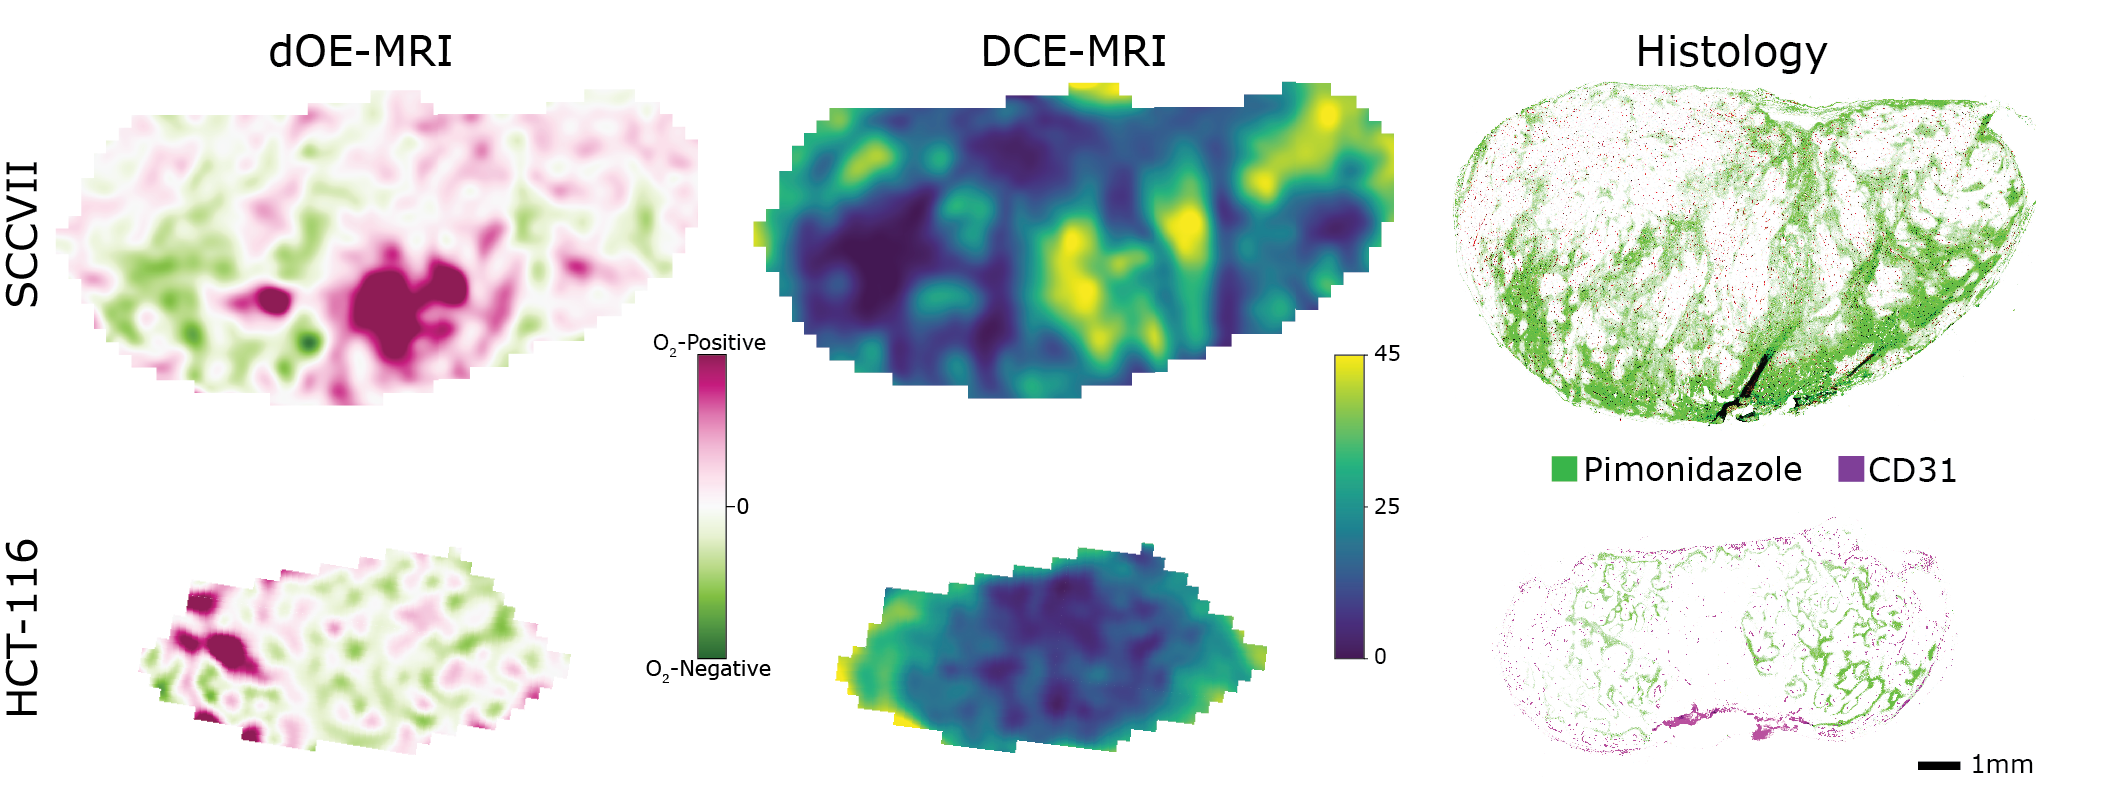
\includegraphics[width=\textwidth]{futurework/futurework-images/fig_perfusion.png} % requires the graphicx package
   \caption{\ac{dOE-MRI} maps and DCE-MRI \acs{AUC}$_{60}$maps and slice-matched histology sections of SCCVII and HCT-116 tumours. Large regions marked as purple in the \ac{dOE-MRI} maps are O$_2$-positive and also correspond to regions that have high \acs{AUC}$_{60}$ values (yellow). Green or O$_2$-negative regions from the \acs{dOE-MRI} map are often consistent with unperfused regions in the \acs{AUC}$_{60}$ (black), but there are regions of mismatch. Histology images stained with pimonidazole (green) and CD31 (purple) are shown for corresponding sections.
   \label{fig_perfusion}}
\end{figure}

\section{Expanding \texorpdfstring{\acs{dOE-MRI}}{dOE-MRI} to include \texorpdfstring{T$_2^*$}{T2*}}
\label{futurework:expandingdOEMRI_T2*}
%%% from the grant

For a variety of reasons, the past 5-10 years have seen a gradual resurgence of oxygen-enhanced MRI and renewed interest to refine and better understand the mechanism of action.
One important strategy to elucidate the mechanism of oxygen as a contrast agent is to rely on the \acs{BOLD} effect. 
Little et al.\ have recently shown that simultaneous acquisition of T$_1$ and T$_2^*$ images improves the specificity of oxygen-enhanced MRI~\cite{Little:2018iu}.
Here we outline how our technique using \acs{ICA} can be expanded to include T$_2^*$ imaging, and what the additional information will be used for.

T$_2^*$ imaging would utilize the Blood Oxygen Level Dependent (\acs{BOLD}) effect, which can measure shifts in hemoglobin saturation through changes in T$_2^*$ and therefore assess tumour perfusion without the need for injectable contrast agents. 
Applying an oxygen challenge also shifts the haemoglobin saturation and, thus, the T$_2^*$ signal. 
The expected behaviour of a joint change in T$_1$ and T$_2^*$ in response to a gas challenge, and how this can be interpreted to reflect tumour oxygenation is based on data from recent work by Little~\cite{Little:2018iu} and Waterton et al.~\cite{OConnor:2019fc}. 

The altered T$_2^*$ provides a robust measure of areas with functioning vasculature. 
Subsequently, \acs{dOE-MRI} maps can be masked using the $\Delta$T$_2^*$ maps to exclude unperfused regions and enable improved \acs{SNR} for T$_1$-weighted signals, resulting in a completely endogenous technique to assess tumour oxygenation. 
OE-MRI T$_1$-weighted signal more directly reflects oxygen amounts in plasma and tissues and is more applicable for measuring tumour oxygenation as it relates to radiotherapy.
Without sacrificing the information obtained from T$_1$-weighted signal intensity in our current work, we propose to extract both T$_1$-weighted signal intensity and T$_2^*$ simultaneously using a dynamic, multi-gradient echo in place of a dynamic FLASH sequence. 
The cycling gas challenge in combination with \acs{ICA} improvement to T$_1$-weighted oxygen-enhanced imaging will also be applicable to T$_2^*$.

A multi-gradient echo (\acs{MGE}) sequence is ideal to extend our current T$_1$ based dOE-MRI technique to also acquire dynamic T$_2^*$ weighted data.
This is because initial echoes from an \acs{MGE} sequence are T$_1$ weighted and as the echo time increases, the images become more T$_2^*$ weighted. 
The T$_1$w \acs{dOE-MRI} map can be calculated from the signal intensity of the first gradient echo image (minimal echo time TE$\approx$2.25 ms). 
The T$_2^*$ \acs{dOE-MRI} map can be created by applying \acs{ICA} to the mono-exponentially fitted multi-gradient echo data at each repetition. 
Figure~\ref{MGE_schematic} outlines our approach to obtain T$_1$- and T$_2^*$-based \acs{dOE-MRI} maps from a single multi-gradient echo sequence. 
While the temporal resolution of the multi-gradient echo technique is lower, the data quality of the T$_1$w \acs{dOE-MRI} map is not compromised until subsampling exceeds six times the original temporal resolution when compared to that obtained with a \acs{FLASH} sequence (see Figure~\ref{sec:interleave}).

\begin{figure}[htbp]
   \centering
   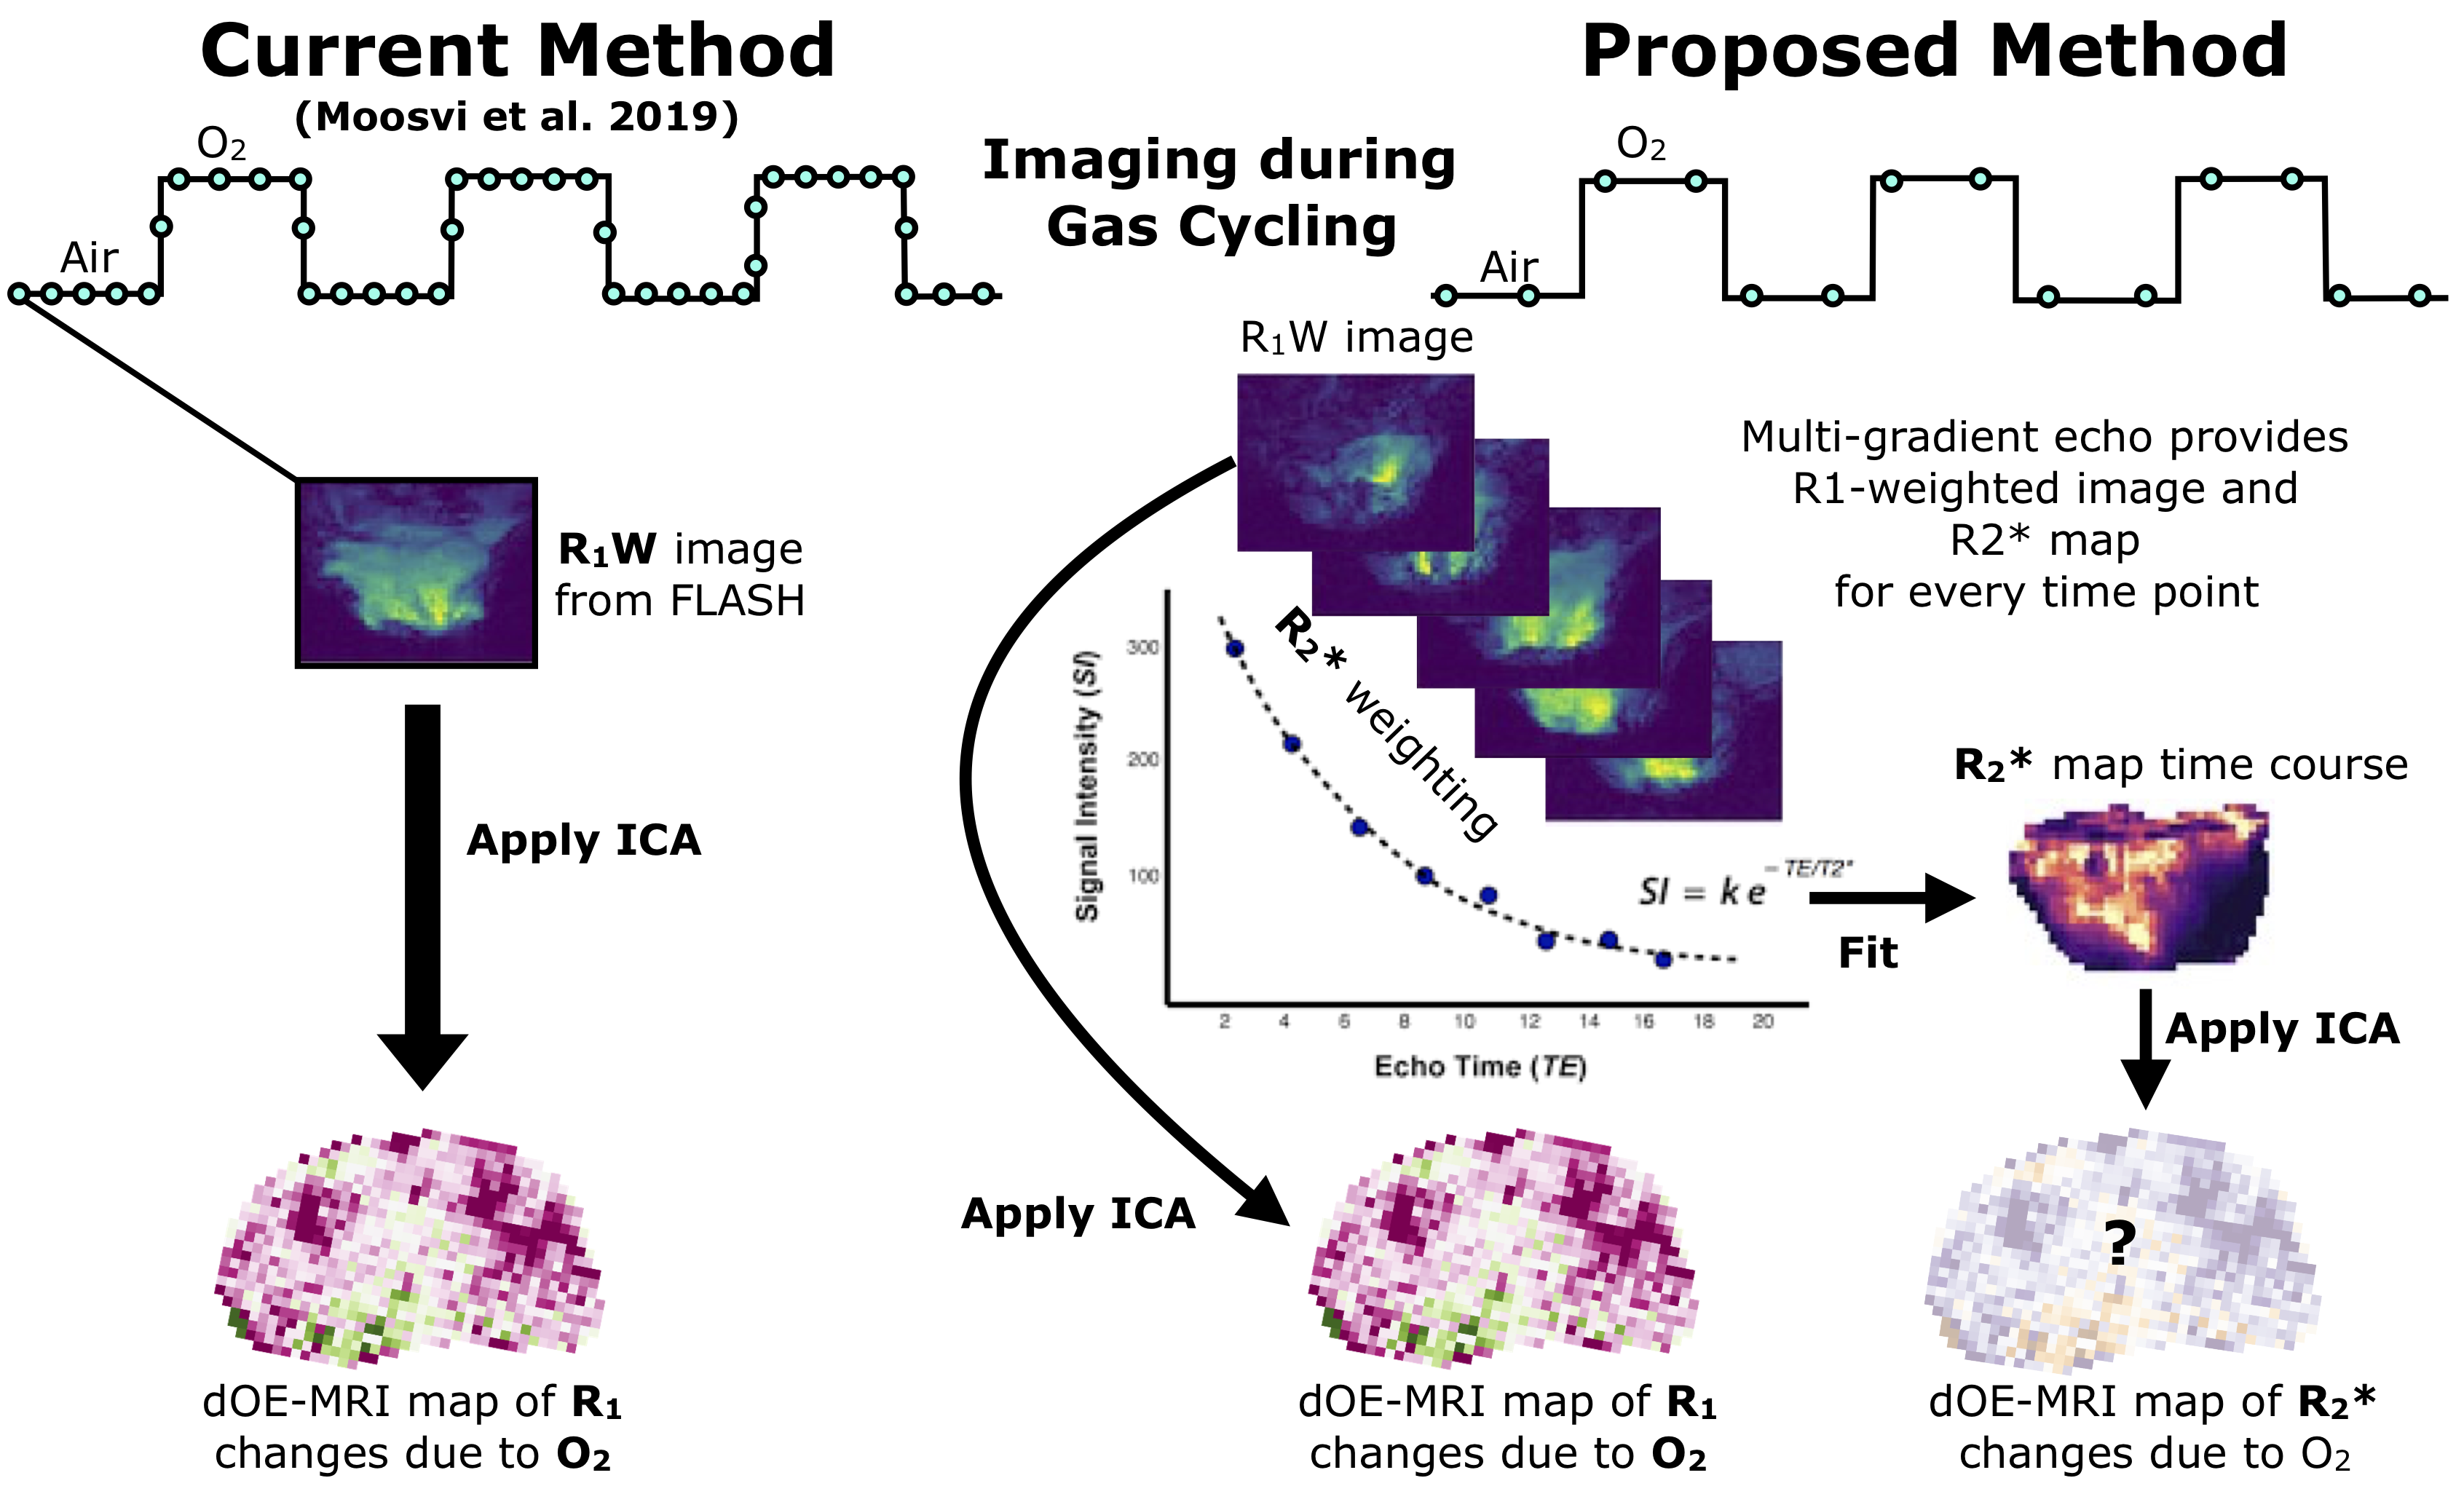
\includegraphics[width=\textwidth]{futurework/futurework-images/grantfig4_MGE_schematic.png} % requires the graphicx package
   \caption{Schematic of the current and proposed acquisition and analysis for \acs{dOE-MRI} with combined R$_1$ and R$_2$ imaging.
   \label{MGE_schematic}}
\end{figure}

\subsection{Independent Vector Analysis}

\acs{ICA} can be extended if the data being analyzed is multi-dimensional beyond temporal and spatial coordinates, for instance, T$_1$ and T$_2^*$ weighted images.
Independent vector analysis (\acs{IVA}) is the technique that permits the increased statistical power of two independent parameters acquired simultaneously.
It is a vector-based blind-source estimation first used in \acs{fMRI} applications~\cite{Lee:2008dc}. 
The problem solved by \acs{IVA} is that observations that are vector quantities (i.e. data consisting of one T$_1$-weighted signal and one T$_2^*$ value derived from the exponential fit) are explained by a mixture of source vectors~\cite{Lee:2008dc}:

\begin{equation}
x_i = \sum_{j}^{L} a_{ij} \circ s_j
\end{equation}

where $\circ$ indicates an element-wise product. 
An algorithm suggested by Rafique et al.\ in 2016 solves the implementation problem and makes it available as FastIVA~\cite{Rafique:2016cf}.
It would be worthwhile to explore \acs{IVA} as an extension to \acs{ICA} once the T$_1$ and T$_2^*$ weighted data is acquired.

%\begin{figure}[htbp]
%   \centering
%   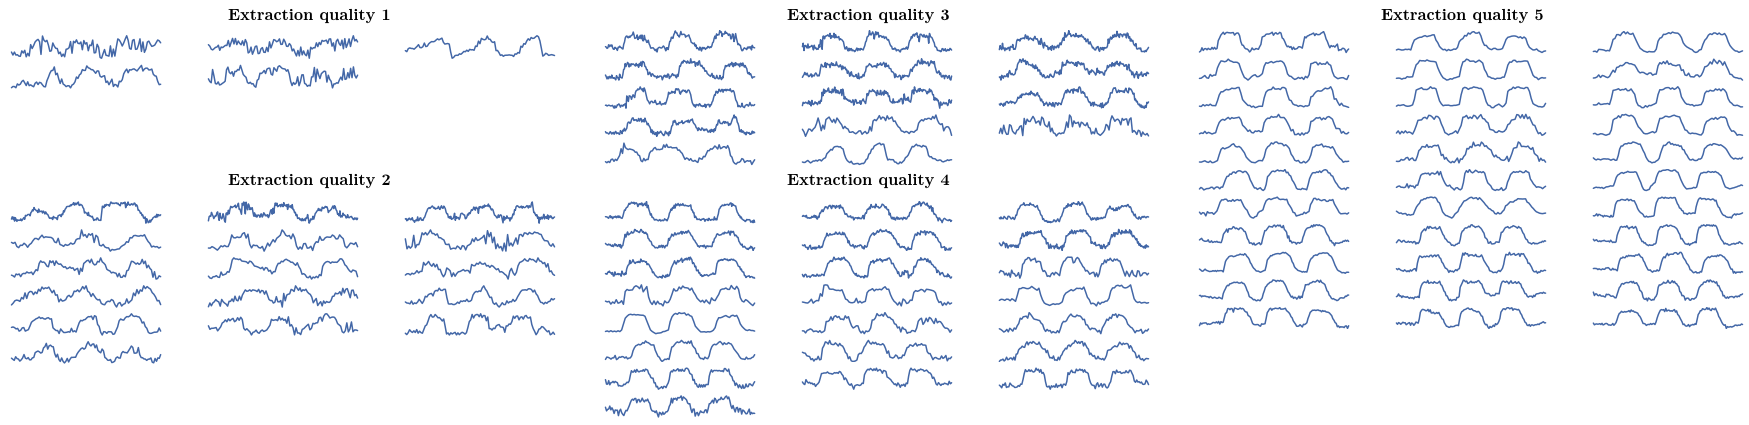
\includegraphics[width=\textwidth]{futurework/futurework-images/technical_ScoredExtractions.png} % requires the graphicx package
%   \caption{Each trace plot is the extracted ICA component corresponding to the oxygen response. The components are scored by the observer from a score of 1 to 5, with 1 barely corresponding to the oxygen challenge with a lot of noise and 5 corresponding extremely well to the oxygen challenge and very little noise. Note very few animals are in the lowest group, and many more are of extraction quality 4 and 5.}
%   \label{extractions}
%\end{figure}





\endinput